\solution{
	Implication graph:\medskip 
	\begin{figure}[ht]
	\centering
	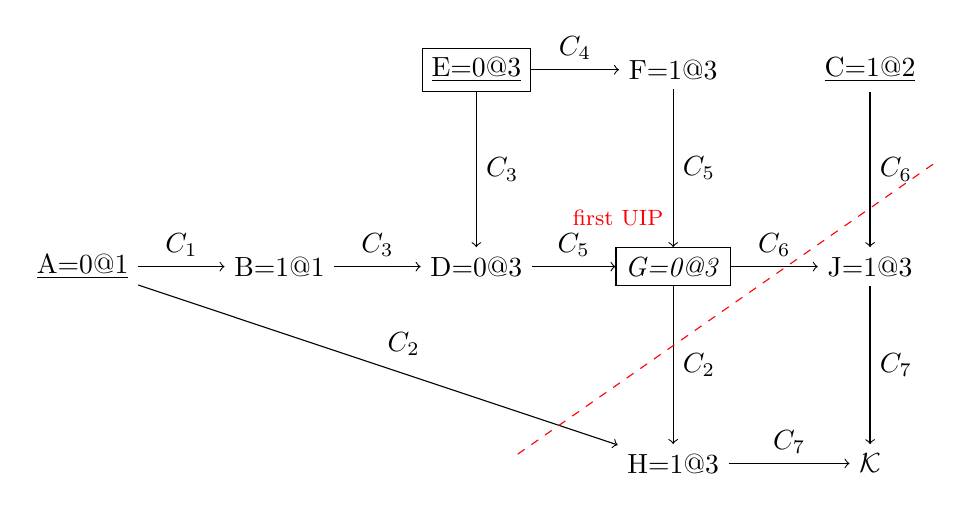
\begin{tikzpicture}[node distance=2.5cm,auto]
	\node (A) {\underline{A=0@1}};
	\node (B) [right of=A] {B=1@1};
	\node (D) [right of=B] {D=0@3};
	%\color{red}
	\node (G) [right of=D, rectangle, draw=black] {\textit{G=0@3}};
	%\color{black}
	\node (H) [below of=G] {H=1@3};
	\node (K) [right of=H] {$\mathcal K$};
	\node (E) [above of=D, rectangle, draw=black] {\underline{E=0@3}};
	\node (F) [right of=E] {F=1@3};
	\node (J) [right of=G] {J=1@3};
	\node (C) [above of=J] {\underline{C=1@2}};
	\path[->] (G) edge node {$C_6$} (J);
	\path[->] (F) edge node {$C_5$} (G);
	\path[->] (C) edge node {$C_6$} (J);
	\path[->] (J) edge node {$C_7$} (K);
	\path[->] (E) edge node {$C_3$} (D);
	\path[->] (E) edge node {$C_4$} (F);

	\path[->] (A) edge node {$C_1$} (B);
	\path[->] (B) edge node {$C_3$} (D);
	\path[->] (D) edge node {$C_5$} (G);
	\path[->] (G) edge node {$C_2$} (H);
	\path[->] (H) edge node {$C_7$} (K);
	\path[->] (A) edge node {$C_2$} (H);

	\node [above,red] at (6.8,0.4) {{\footnotesize \textrm{first UIP}}};
	\draw [red,dashed](10.8,1.3) -- (5.5,-2.4);
	\end{tikzpicture}
	\label{pic:impl_graph}
	\caption{{\protect\small Implication graph with UIPs (nodes with
	rectangles), where the second rectangle node ($G$) with the cursive label
	denotes the \textit{first UIP}.}}
	\end{figure}
	\newline
	%Implication Graph with first UIP (red) and the corresponding cuts (dashed).

	\bigskip

	We have a conflict in $c_{7}$, since $\lnot J$ and $\lnot H$ are not
	satisfied. So we have to resolve and backtrack to the first UIP, which is $%
	G=0@3$.

	Since $c_{2}$, $c_{6}$ and $c_{7}$ are conflict clauses along the out-edges
	and are (the first) on the paths from the first UIP. Hence, the assertion
	clause can be computed, using resolution, as follows:\newline

	% $\tfrac{%
	% \begin{array}{l}
	% c_{2}:A\OR G\OR H \\ 
	% \underline{c_{7}:\lnot J\OR\lnot H}\newline
	% \end{array}%
	% \newline
	% }{c_{8}:A\OR G\OR\lnot J}\tfrac{%
	% \begin{array}{l}
	% c_{6}:\lnot C\OR G\OR J\newline
	% \\ 
	% \underline{c_{8}:A\OR G\OR\lnot J}%
	% \end{array}%
	% \newline
	% }{c_{9}:A\OR\lnot C\OR G}$(after removing the second G with fac.)\newline

	\begin{equation*}
	r_{1}=res(c_{7},c_{2},H)=A\OR G\OR\lnot J\text{\quad and\quad }%
	r_{2}=fac(res(r_{1},c_{6},J))=A\OR\lnot C\OR G.
	\end{equation*}

	The result $r_{2}$ yields the learned clause $c_{8}=(A\OR\lnot C\OR G)$ and
	we backtrack to the highest decision level $DL=3$, i.e. we remove all
	decisions and values at $DL\geq 3$ and change the decision of $E$ to $E=1@3$.

	\medskip

	Thus, we get a new implication graph:\newline

	\begin{figure}[ht]
	\centering
	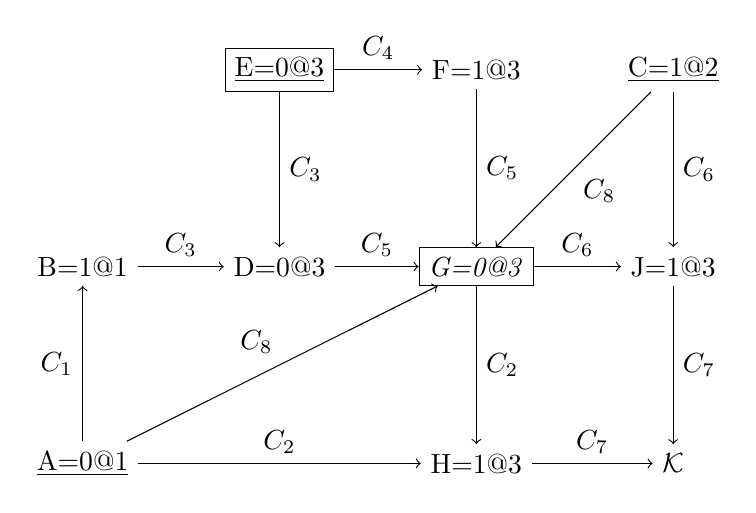
\begin{tikzpicture}[node distance=2.5cm,auto]
	\node (B) {B=1@1};
	\node (A)[below of=B] {\underline{A=0@1}};
	\node (D) [right of=B] {D=0@3};
	\node (G) [right of=D, rectangle, draw=black] {\textit{G=0@3}};
	\node (H) [below of=G] {H=1@3};
	\node (K) [right of=H] {$\mathcal K$};
	\node (E) [above of=D, rectangle, draw=black] {\underline{E=0@3}};
	\node (F) [right of=E] {F=1@3};
	\node (J) [right of=G] {J=1@3};
	\node (C) [above of=J] {\underline{C=1@2}};
	\path[->] (G) edge node {$C_6$} (J);
	\path[->] (F) edge node {$C_5$} (G);
	\path[->] (C) edge node {$C_6$} (J);
	\path[->] (J) edge node {$C_7$} (K);
	\path[->] (E) edge node {$C_3$} (D);
	\path[->] (E) edge node {$C_4$} (F);

	\path[->] (A) edge node {$C_1$} (B);
	\path[->] (B) edge node {$C_3$} (D);
	\path[->] (D) edge node {$C_5$} (G);
	\path[->] (G) edge node {$C_2$} (H);
	\path[->] (H) edge node {$C_7$} (K);
	\path[->] (A) edge node {$C_2$} (H);

	\path[->] (C) edge node {$C_8$} (G);
	\path[->] (A) edge node {$C_8$} (G);
	\end{tikzpicture}
	\label{pic:new_impl_graph}
	\caption{{\protect\small New implication graph with UIPs (nodes with
	rectangles) and the learned clause $c_{8}$.}}
	\end{figure}

	The learned clause $c_{8}$ implies that the node $G$ must be set to $1@3$,
	else $c_{8}$ would be unsatisfied and we get again a new conflict. This
	implies in turn, that the value either in $D$ or in $F$ can be arbitrarily
	chosen. This is also the case for node $J$ and node $H$. One of both nodes
	the value can be arbitrarily chosen and the ohter must be set to $0@3$. By
	setting $F=H=0@3$, we observe that all clauses $c_{i}$, $i\in \{1,\ldots
	,8\} $ are satisfied and obtain a model $M=\{\lnot A,B,C,D,E,F,G,\lnot H,J\}$%
	.

	% \begin{tikzpicture}[node distance=2.5cm,auto]
	% \node (A) {A=0@1};
	% \node (B) [right of=A] {B=1@1};
	% \node (C) [right of=B] {C=1@2};
	% \node (E) [right of=C] {E=1@3};				
	% \path[->] (A) edge node {$c_1$} (B);
	% \end{tikzpicture}
	% \newline
	% \newline
	% The remaining clauses $c_2$, $c_5$, $c_6$ and $c_7$ doesn't contain any
	% rules for the implication graph, so we have to introduce a new decision
	% level $DL 4$ and we can choose the decision for e. g. $G$ as $G = 1@4$:%
	% \newline
	% \bigskip

	% \begin{tikzpicture}[node distance=2.5cm,auto]
	% \node (A) {A=0@1};
	% \node (B) [right of=A] {B=1@1};
	% \node (C) [right of=B] {C=1@2};
	% \node (E) [right of=C] {E=1@3};	
	% \node (G) [right of=E] {G=1@4};			
	% \path[->] (A) edge node {$c_1$} (B);
	% \end{tikzpicture}
	% \newline
	% \newline
	% Again, the remaining clauses $c_5$ and $c_7$ doesn't contain any rules for
	% the implication graph, so we have to introduce a new decision level two
	% times ($DL 5$ and $DL 6$) and we can choose the decisions for e. g. $D$ as $%
	% D = 1@5$ and $H$ as $H = 0@6$:\newline
	% \bigskip

	% \begin{tikzpicture}[node distance=2.5cm,auto]
	% \node (A) {A=0@1};
	% \node (B) [right of=A] {B=1@1};
	% \node (C) [right of=B] {C=1@2};
	% \node (E) [right of=C] {E=1@3};	
	% \node (G) [right of=E] {G=1@4};	
	% \node (D) [below right of=A] {D=1@5};
	% \node (H) [below right of=C] {H=0@6};		
	% \path[->] (A) edge node {$c_1$} (B);
	% \end{tikzpicture}
	% \newline

	% Now we have fulfilled all clauses $c_{i}$, $i\in \{1,...,9\}$ and therefore
	% we can choose any dedcisions for the ramaining values.\newline
	% A valid solution model would be: $\{\lnot A,B,C,D,E,F,G,\lnot H,J\}$

	\bigskip
}